\section{Virtual Work}

%Lectures 34 and 35
A force does work when it produces a displacement along its line of action. 

Virtual work ($dU$) is the work produced by a force over an infinitesimally small displacement $dr$.

\[dU = F\cdot dr\]

Virtual work of a couple moment: 

\[dU = \Vec{M}\cdot d\theta \Vec{k}\]

\begin{figure*}[!h]
\centering
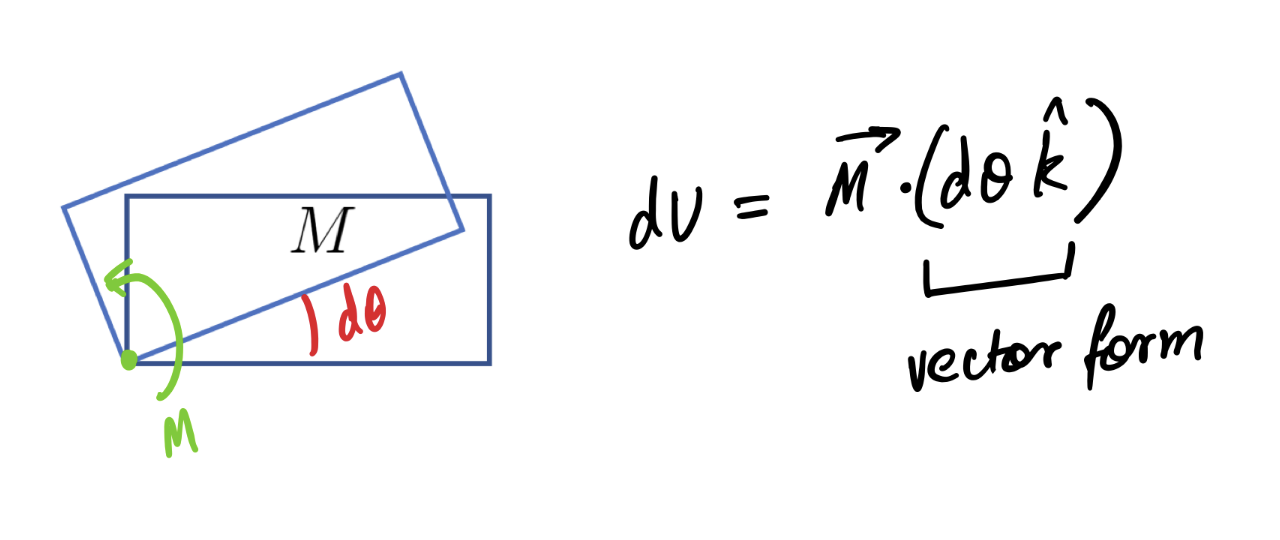
\includegraphics[angle=0, width=5 in]{VWorkFigures/VWorkCoupleMoment.png}
\vspace{-2mm}
\caption{\small Virtual work $dU$ completed by a couple moment, $M$. \blue{Need to add a coordinate system to this picture. Taken from lecture 34.}}
\vspace{-3mm}
\label{Fig:VWorkCoupleMoment}
\end{figure*}

We can use virtual work to solve for the forces in a system without needing to solve for all of the support reactions. For example, if a truss is completely pinned on one end, it doesn't move, which means there is no virtual work completed on that pin because there are no virtual displacements!

\subsection{Virtual displacements}
A virtual displacement is an infinitesimally small displacement (or rotation) that is possible in the system, denoted usually as $dx$ or $d\theta$. It's important to note that virtual displacements are assumed to be possible but don't actually exist. 

\subsection{Principle of Virtual Work}

If a body is in equilibrium, the sum of the virtual work done by all the forces and couple moments acting on the body is zero. 

\begin{figure*}[!h]
\centering
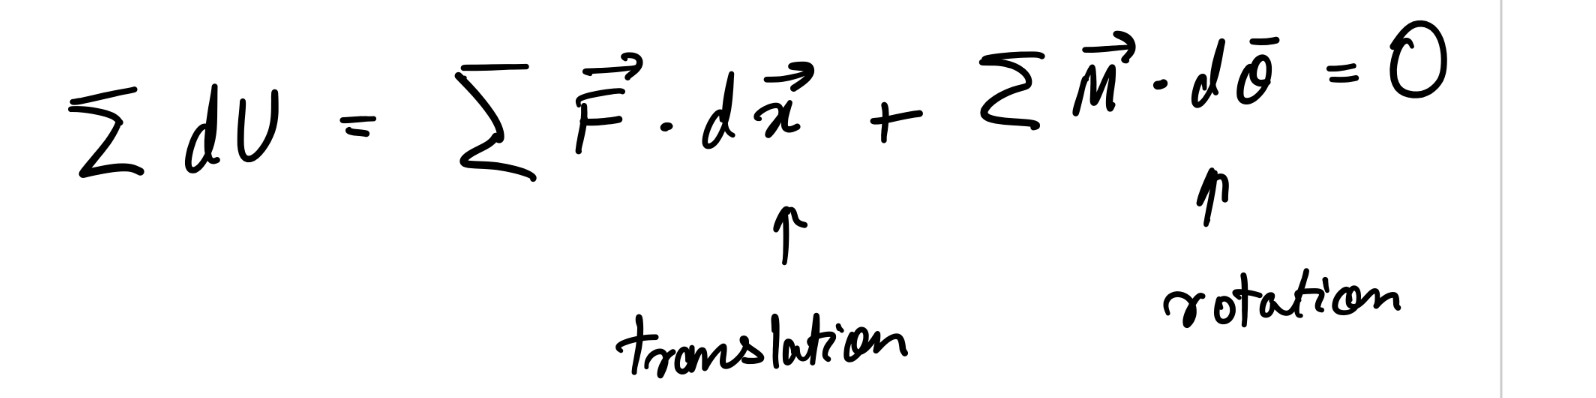
\includegraphics[angle=0, width=5 in]{VWorkFigures/PVW.png}
\vspace{-2mm}
\caption{\small Principle of virtual work. \blue{Taken from lecture 34.}}
\vspace{-3mm}
\label{Fig:PVW}
\end{figure*}

\subsection{Virtual work analysis}

\begin{figure*}[!h]
\centering
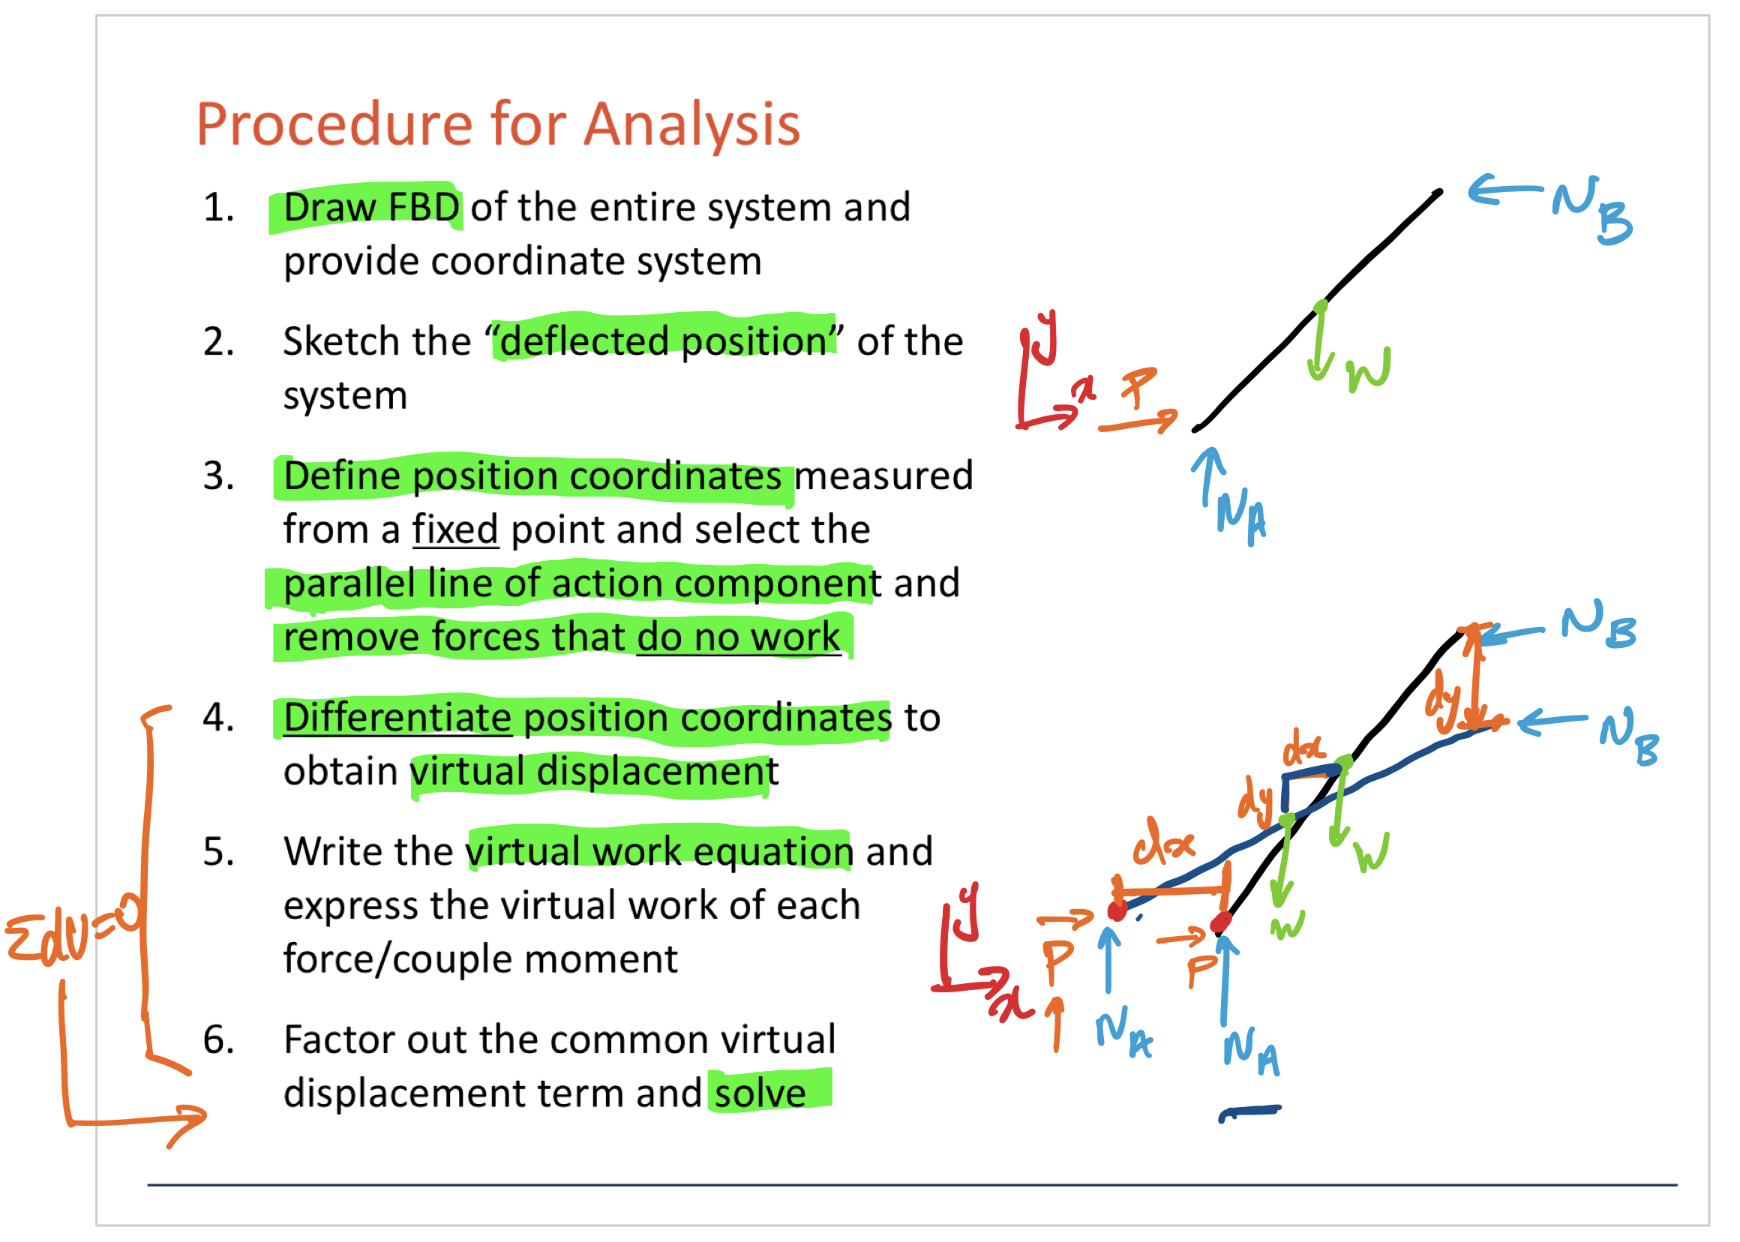
\includegraphics[angle=0, width=5 in]{VWorkFigures/VWAnalysis.png}
\vspace{-2mm}
\caption{\small Analysis procedure for virtual work problems. \blue{Taken from lecture 34.}}
\vspace{-3mm}
\label{Fig:PVW}
\end{figure*}